\chapter{Introduction}
\section{Background}
The $n$-body problem is a class of problems in physics that, in a highly general sense, consists of modelling the motion of $n$ objects interacting through some physical force. In classical mechanics the equations of motion for $n$ point particles can be derived from Newton's second law of motion, which states that the rate of change in momentum for an object equals the force acting on it, or from analytical formulations such as Lagrangian and Hamiltonian mechanics, which consider scalar properties of motion like kinetic and potential energies. In the quantum regime, where the wave-like property of matter has to be taken into account, the state of an $n$-body system is described by a total wave function, where the Hamiltonian operator generates the time evolution of the state as given by Schr{\"o}dinger's differential equation.

The core of the $n$-body problem is that neither the classical equations of motion nor the Schr{\"o}dinger equation are analytically solvable for more than two interacting particles. Consider the case where $n=3$. Although apparently simple, the configuration space for the three-body problem is six dimensional after separating out the center of mass motion. Three additional constants of motion can be provided by conservation of the total angular momentum, which effectively reduces the problem to that of three coupled second order non-linear differential equations in the classical case and a three dimensional Schr{\"o}dinger equation in the quantum case. 

The quest for a general solution to the classical three-body problem is renowned. As a recurrent muse to a number of great mathematicians during the past centuries, dating back to Newton himself, the three-body problem has been a catalyst for the development of analysis and the modern theory of dynamical systems \cite{Chenciner2015}. Although there are a number of special cases that have explicit solutions, non-linear dynamical systems often display highly unpredictable behaviour due to sensitive dependencies on initial conditions, i.e., are chaotic. Nowadays, different numerical approaches are used to solve these kinds of problems, but the computational load can be substantial. 

In contrast to the classical case, the quantum three-body problem is amenable to qualitative analysis \cite{efimov1990qualitative} and in some cases, even to analytic solutions. In the quantum realm of few-body systems the Faddeev and the Faddeev-Yakubovsky equations, which are equivalent formulations of the Schr{\"o}dinger equation for three- and four-body systems respectively, can, for a few special cases, be solved analytically by iteration \cite{Faddeev:1960su, Zubarev:1994}. For the three-body scattering problem bound state solutions can exist in cases where all three two-body subsystems have short-ranged interactions, if at least two of these interactions are close to resonance. This is called the Efimov effect. 

\section{The Birth of Efimov Physics}
In low energy scattering, particles are said to resonate when the strength of the attractive interaction between them barely cancels out the repulsive effect of the kinetic energy. During the collision they remain close for an extended period of time, in an almost bound state, before separating. 

In 1970, Vitaly Efimov predicted that resonant two-body forces could give rise to a series of bound energy levels in three-particle systems \cite{Efimov:1970zz}. When the short-ranged two-body forces approached resonance, he found a universal long-range three-body attraction emerging, giving rise to an infinite number of trimer states with binding energies obeying a discrete scaling law at resonance.  

Efimov proposed that attractive three-body interaction appearing in systems with resonant short-ranged interactions and repulsive Coulomb forces could explain the binding of three particle nuclei such as the three nucleon triton $\prescript{3}{}{\mathrm{H}}$ and the triple-alpha Hoyle state of $\prescript{12}{}{\mathrm{C}}$ \cite{Efimov:1970zz,Efimov:1971zz}.

The notion of Efimov physics comprises a range of universal phenomena that occur in few-body systems exhibiting the Efimov effect. Short-ranged forces commonly occur in nature and few-body effects are expected to appear in a broad range of physical systems. Development in the theory of few-body quantum systems is important, since it could bridge the gap between existing well developed models of treating one- and two-body systems and the statistical methods used to describe many-body systems.

\section{Theoretical Introduction}
A short review concerning some important aspects of quantum mechanical systems and two-body scattering, in particlular the concept of \emph{scattering length}, will follow, in order to set the stage for a discussion of quantum effects in few-body systems in general and Efimov states in three-body systems in particular. A more detailed description of two-body scattering will be given in \cref{chap:3}.

\subsection{Entering the Quantum Realm}
All particles of matter exhibit wave-like properties. The wavelength of a particle with momentum $p$ is given by the de Broglie equation

\begin{equation} \label{eq:1}
\lambda = \frac{h}{p} = \frac{h}{mv}
\end{equation}
where $h$ is the Planck constant. The wave characteristics of matter grow with increasing de Broglie wavelength. When the wavelength is sufficently large, classical physics no longer applies and the system has reached the quantum regime. From \ref{eq:1} it is evident that this is true for particles that are very small or very slow. In an ultracold quantum gas, the atoms are cooled down to a point where they move so slowly that the increased uncertainty in position for the individual atoms becomes so large that they start to overlap with each other. At this point the atoms can not be viewed as individual particles but as a correlated wave. The de Broglie wavelength of the atoms is then larger than the average interatomic spacing, which is typically about one micron in a low density gas, and their behaviour is fully governed by quantum mechanics. In other words, the transition to the quantum regime occures when the thermal de Broglie wavelength is on the order of the interparticle spacing. Since the temperature of the gas and the thermal de Broglie wavelength are related through

\begin{equation}
\lambda = \frac{h}{\sqrt{2\pi m k_B T}},
\end{equation}
in which $k_B$ is the Boltzmann constant, it means that there is a critical temperature for when the quantum effects become dominant. For a dilute atomic gas this critical temperature is in the microkelvin to nanokelvin range.

\subsection{Two-body Interactions}
Atomic interactions are pair-wise and short ranged, which means that they interact when they are close to each other. At sufficently low energies, atoms behave like point particles and have quantized orbital angular momenta $l$. In analogy with atomic orbitals, the quantum numbers $l=0,1,2,$ associated with an atom, are referred to as $s$-waves, $p$-waves and $d$-waves, respectively. 

The scattering processes of two particles can be decomposed into that of an incoming plane wave, expanded into a sum of partial waves with definite angular momenta, which scatters off a potential placed at the origin. For low energy scattering, only the first few $l$-quantum numbers contribute to the scattering process and in the ultracold regime $s$-wave collisions dominate. Scattering becomes isotropic when the wavelength of the relative particle is much larger than the typical interparticle interaction range $r_0$, since the wave is then too large to resolve the details of the short-range interaction. In other words, the colliding atoms cannot resolve each other's internal structure provided by their electron configurations. This makes scattering in the low energy limit indistinguishable from that of point particles. Furthermore, only spherical waves will come close enough to be scattered by the potential. Higher partial waves ($l>0$) will not ``feel'' the potential since they will be reflected by a centrifugal barrier at separations greater than the interaction range. Two-body scattering in this regime is solely governed by a single parameter called the $s$-wave scattering length $a$. The $s$-wave scattering length, referred to as `the scattering length' from here on, is defined in the low-energy limit as

\begin{equation} \label{eq:2}
a = \lim_{k \to 0} -\frac{\tan\delta_0(k)}{k},
\end{equation}
where $k$ is the wave number ($k=p/\hbar = \sqrt{2\mu_{2b} E}/\hbar$), $\mu_{2b}$ is the two-body reduced mass and $\delta_0(k)$ is the $s$-wave phase shift of the outgoing wave. For small $k$, the phase shift will behave as $\delta(k)\approx-ka + O(k^2)$. If scattering by a hard sphere is considered, the scattering length $a$ is simply the radius of the sphere. In the low energy limit, the scattering properties for an arbitrary potential is the same as that of a hard sphere with radius $a$. Scattering can therefore occur at separations greater than the interaction range if the magnitude of the scattering length is sufficently large. The scattering length characterizes the strength of the short-range interparticle interaction. Since a positive scattering length corresponds to a negative phase shift, which means that the scattered wave is pushed out, the effective interaction will be repulsive and an increase in $a$ will cause the underlying attractive potential in a two-body bound state to become less attractive. Increasing the magnitude of a negative scattering length will, on the other hand, make the potential more attractive, since the phase shift is now positive and the scattered wave is pulled in, see \cref{fig:phaseshift}. Even though the effective interaction is attractive at negative scattering lengths, the interaction will always be to weak to support a two-body bound state.  

\begin{figure}
	\centering  
	\subfigure[The wave function is pushed outwards when the magnitude of a positive scattering length is increased.]{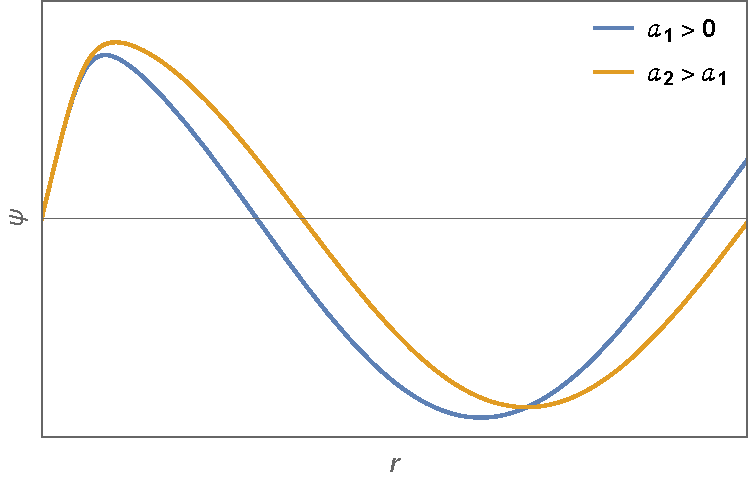
\includegraphics[width=0.45\linewidth]{pos_scat.pdf}}
	\subfigure[The wave is pulled inwards when the magnitude of a negative scattering length is increased.]{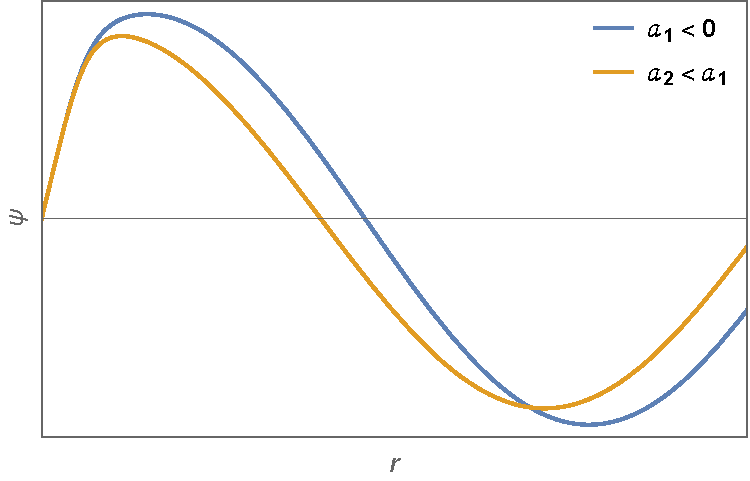
\includegraphics[width=0.45\linewidth]{neg_scat.pdf}}
	\caption{Illustration of the phase shifts causing the effective interaction and how they depend on the sign and magnitude of $a$.}\label{fig:phaseshift}
\end{figure}
In the abscence of an interaction, the phase shift is simply zero. The strongest dephasing occurs when $\delta_0$ takes the value $\pi/2 \pmod{\pi}$, whereupon two-body $s$-wave resonances are formed. This situation is of particular interest in this thesis because Efimov physics arises when the two-body interactions are near resonance. Since the phase shift for the $s$-wave can be written as $\delta_0 \propto -ka$ in the long wavelength limit ($k \ll r_0^{-1}$), it means that the scattering length $a$ has to become much larger in magnitude than the interaction range $r_0$ for a two-body interaction to become resonant.

\subsection{Universality}
Particles with large scattering lengths, i.e., $\abs{a}\gg r_0$, in the low-energy regime have universal properties. The properties are universal in the sense that they depend on the scattering length alone and not on the details of the short-range interaction. Alkali atoms interact via van der Waals potentials of the form $-C_6/r^6$, where the range $r_0$ is typically on the order of the van der Waals length, which can be defined by \cite{vanderWaals}

\begin{equation}
l_{vdW} = \frac{1}{2}\bigg(\frac{2\mu_{2b} C_6}{\hbar^2}\bigg)^{1/4}.
\end{equation}

For a system of two identical bosons with $a>0$, there is a universal shallow two-body bound state near the scattering threshold, with binding energy 
\begin{equation}\label{shallowdimer}
E_D = \frac{\hbar^2}{2 \mu_{2b} a^2}.
\end{equation}
For $a<0$ there is no such bound state. Outside the universal range the natural binding energy for two particles should be approximately $1/mr_0^2$. The cross section for elastic scattering of two identical bosons in this regime is also universal and so is the mean square radius, which are given by

\begin{equation}\label{elasticcross}
\sigma = 8\pi a^2
\end{equation}
and

\begin{equation}\label{meanradius}
\langle r^2\rangle = \frac{a^2}{2},
\end{equation}
respectively. The universal quantities given in \crefrange{shallowdimer}{meanradius} are exact for $a=\pm \infty$ and approximate for $\abs{a}\gg r_0$. The unique dependence on this one length parameter also leads to continuous scaling symmetries in these quantities. If the scattering length is scaled with some real factor $\lambda$ such that $a \to \lambda a$, the shallow dimer energy will scale as 

\begin{equation}
E_D(\lambda a) = \lambda^{-2}E_D(a),
\end{equation}    
while the elastic cross section and the mean square radius scale as 

\begin{equation}
\sigma_e(\lambda^{-2}k,\lambda a) = \lambda^2 \sigma_e(k,a)
\end{equation}
and

\begin{equation}
\langle r^2(\lambda a)\rangle = \lambda^2 \langle r^2(a)\rangle ,
\end{equation}
respectively. 

While the scattering length completely governs the low energy two-body collision problem, it is also the main parameter for describing the interaction of particles at very low collision energies in general. 

Similarly to the universal quantities found in the two-body sector, three-body systems can also exhibit universal properties. For particles interacting through short-ranged interactions near resonance, i.e., when the attraction is on the verge on, or can just bareley support a shallow dimer, an effective long-range three-body attraction emerges, which can form shallow three-body bound states with binding energies $E_T^n$ that scale geometrically in the trimer region, see \cref{fig:efimov}. To understand how this long-range interaction is formed, consider a collision between the shallow dimer and a third particle in the low energy limit. The third particle will start to ``feel" the dimer when it comes close to the two-body scattering length $a$, which is also the size of the dimer. At this point the third particle could tug off any of the particles in the dimer to form a new pair. It is this process of particle exchange that results in the effective three-body interaction that Vitaly Efimov found when he was studying the quantum three-body problem. This effective long-range attraction is universal in the sense that it emerges irrespective of the underlying two-body short-range interactions. The scaling in this sector is discrete. The infinite ladder of energy levels that appear in the asymptotic limit when $a \to \pm \infty$ have a discrete geometric scaling symmetry. The size of an excited state is larger than the previous state by a factor of $\lambda = e^{\pi/s_0} \simeq 22.7$. The scaling law applies radially see figure bla bla %TODO. The energy of the excited state scale like

\begin{equation}
\frac{E_T^{n+1}}{E_T^{n}} = e^{2\pi/s_0}
\end{equation}

\begin{equation}
N \approx \pi^{-1} \ln(\abs{a}/r_0)
\end{equation}

\begin{figure}
	\centering
	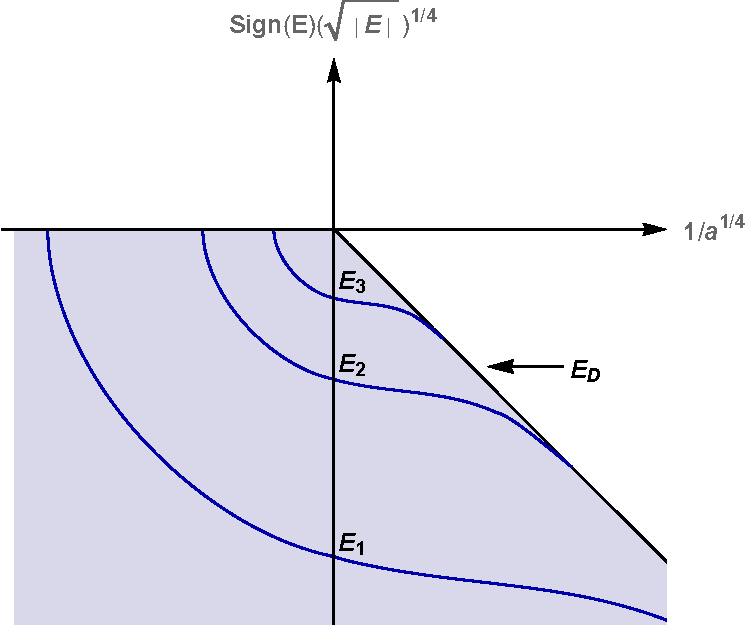
\includegraphics[width=0.75\linewidth]{efimov}
	\caption{The energies of the three first Efimov states are plotted as  functions of the inverse scattering length $a$. Three different regions can be identified in the figure. The three atom continuum is the region above the zero-energy threshold. The atom-dimer region is the region enclosed by the horisontal axis and the atom-dimer threshold and the trimer region shown in grey, in which Efimov states are represented by the blue lines.\cite{Kajsa_my}}\label{fig:efimov}
\end{figure} 
